\chapter{Implementation}
As evaluated in the last sections we will proceed to implement TF-DAC-MACS with small adaptions for a practical secure cloud storage system. To do so the role of the four entities present in the system will be shortly summarized:

\begin{itemize}
  \item \textbf{Central Server} does the initial setup of the global public parameter used in the later process. It publishes this information on a public bulletin board. Further, the CA is the central entry point to trigger and permit AA creations. It audits the \textit{Authority Identifier} (\ac{AID}) provided by the AA and which should be unique in this system. 

Further, the CA functions as a \textit{Certificate Authority}. It issues a certificate for the GID and RSA public keys of the user. This certificate can be revoked so that the user is not able to obtain new secret keys from the AA or other data owners.
The CA is also the central service that provides all necessary information to the client. Such as public attribute keys, encrypted user private attribute keys and certificates.
 The Central Server is honest-but-curious.
  \item \textbf{Attribute Authority (\ac{AA})} creates the secret keys for its attributes. Attributes are prefixed with the \ac{AID} to ensure uniqueness among the attribute universe. They have decryption power in their domain. Further, they are in charge of revoking attributes. 
  \item \textbf{Cloud Storage Provider (\ac{CSP})} The cloud storage provider provides storage to save the encrypted files. If an cipher text update is needed the CSP updates the cipher text accordingly. 
  \item \textbf{Users} download and decipher ciphertext. They receive attribute secret keys from the AA, GID and certificates from the server and two factor keys from the data owners. The CSP is honest-but-curious as well.
  \item \textbf{Data owner} are specifications of users who can issue two-factor keys to other users. The so called \textit{Two-Factor Key} (\ac{2FA}-Key), adds an additional security layer to the cipher text. It restricts the access to the encrypted plain text to a even smaller select user group.  
\end{itemize}

In the following sections, the different phases setup, encrypt, decrypt, attribute revocation and authentication key revocation are shortly explained. Please note that for any scheme details we referrer to the TF-DAC-MACS \cite{li2017two} paper .

\section{Setup}
The setup summarizes the steps described in \cite{li2017two} such as: Setup, user registration, data owner registration, authority setup, key generation and authentication requests. 

% GPP init
\subsection{Generate Global Public Paramter}
The very first step is to create the global public parameters on the central server. Thous parameter are exposed on a public bulletin board and available for each entity in the system. Since they are required in every step it is assumed that the entity downloaded this information in advance. 

% AA setup
\subsection{Setup Attribute Authority}
\begin{figure}[!h]
\centering
    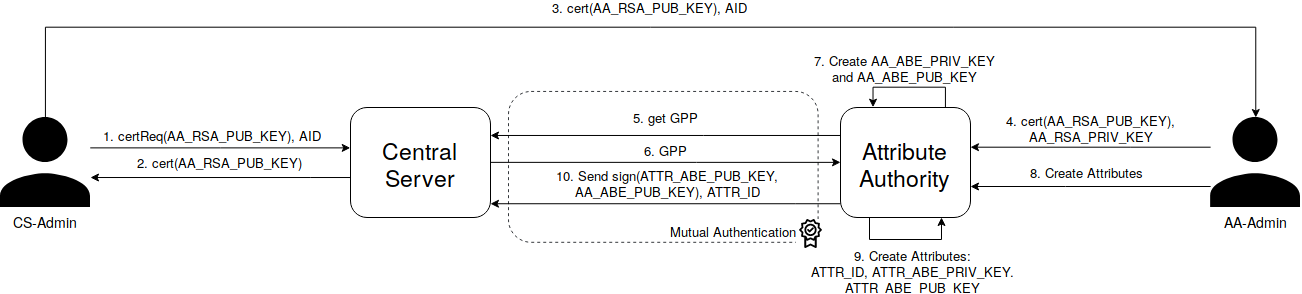
\includegraphics[width=\linewidth]{img/aa_setup.png}
    \caption{Attribute Authority Setup}
    \label{fig:aa-setup}
\end{figure}
An AA is registered, as shown in figure \ref{fig:aa-setup}, with the help of a central server administrator (CS-Admin) and a attribute authority administrator (AA-Admin). As a prerequisite the AA-Admin already created a RSA key pair and send the public component to the CS-Admin together with the desired authority identifier (AID). The AID should be globally unique among this ecosystem so that authority domains can be clearly differentiated. Now the CS-Admin creates a new certificate request embedding the RSA public key of the new AA (1.). The central server checks that the given AID is unique and signs the certificate request (2.). The resulting certificate is passed back to the AA (3.) where it, together with the RSA private key, can be used for mutual certificate authentication. 

The AA-Admin uploads the received certificate and the private key to the AA service (4.) so that it can communicate confident and authenticated with the central server. For each ABE related key generation the GPP are needed, which can now be retrieved over a secured channel, from the CS (5. and 6.). To create attribute keys first an ABE authority key needs to be created (7.) . Now the AA-Admin specifies the attributes by providing the attribute name and values to the service (8.). Internally, the attribute value keys are generated (9.). For each attribute value a ABE key-pair is generated. And to ensure uniques of the attribute identifier it is composed using the following syntax: "<AID>.attr.<Attribute\_name>:<Attribute\_value>". For example the major computer science would be displayed as "aa.tu-berlin.de.attr.major:computer\_sience". In the final step, a signed version of the public attribute value keys and authority public key and the attribute identifier are uploaded to the central service (10.).

\subsection{Register a user}
\begin{figure}[!h]
\centering
    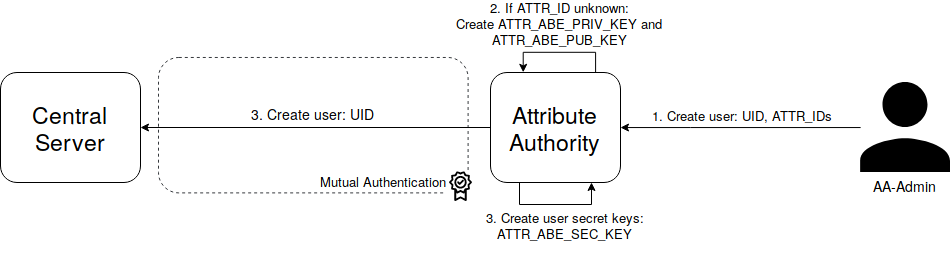
\includegraphics[width=\linewidth]{img/user_register.png}
    \caption{Register a user}
    \label{fig:user-register}
\end{figure}
Figure \ref{fig:user-register} shows the user registration flow. Users are registered by the AA-Admin. He chooses a user identifier (UID) and attributes for the new user (1.).  The AA now checks if all attribute values are already known or if a new attribute value key pair needs to be created (2.). If new attribute values would have been created their public component would also be signed and published to the central server. The user specific attribute secret keys needs to be created (3.). They have the hash of the UID embedded so that on colluding with other users this hash would mesh and no successful decryption would be possible. Finally, the central server is notified for this new user. It just saves the user object for future reference.

\subsection{Register a device}
\begin{figure}[!h]
\centering
    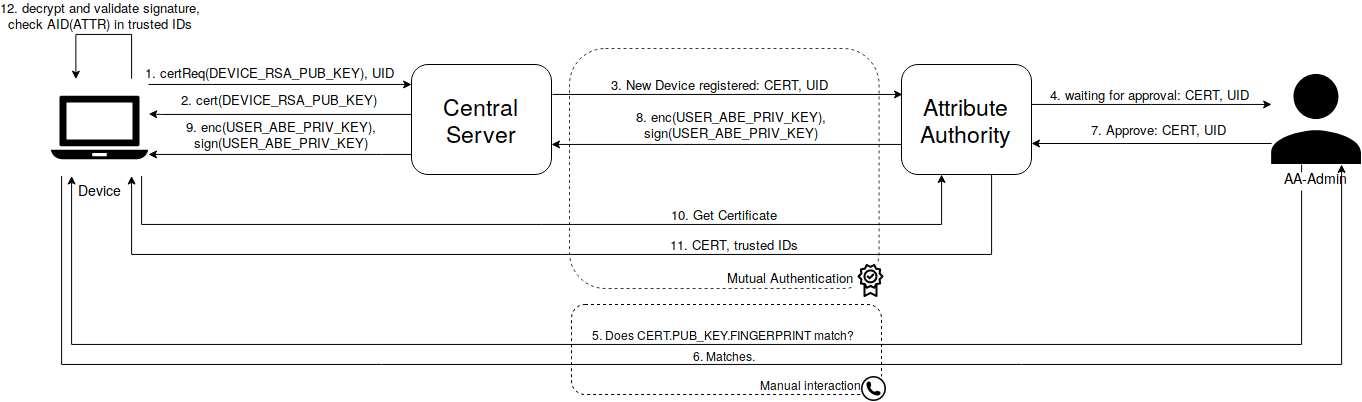
\includegraphics[width=\linewidth]{img/device_register.png}
    \caption{Register a device for a user}
    \label{fig:device-register}
\end{figure}

A device is the first end-system that is able to encrypt and decrypt files in the system. Figure \ref{fig:register-device} shows the rather complex flow for registering a new device. We start off by first creating a new RSA key pair on this device. These are used for later communication and securing the transmission of the private attribute keys to the client. 

The device creates a new certificate request embedding its public key as the subject. This certificate request is posted as a pending request under a user object (1.). The central server processes the certificate request, validates that the user with the desired UID exist and returns a certificate for this request to the device (2.). In addition the central service notifies the AA of the user that a new device was initialized by passing the new certificate (3.). The AA-Admin gets notified for this new device and its certificate (4.). He then manually contacts the addressed user and asks him if he registered a new device (5.). They compare fingerprints of the public key of the certificate and the public key of the user’s device (6.). If they match the AA-Admin approves the device (7.). The AA encrypts the attribute secret keys of the user with the public key embedded in the certificate, signs the content and pushes this information to the central server (8.). 

The double check between AA-Admin and user is imported because the central service (since it might try to provide wrong information) might have generated a new RSA key pair, self-signed the certificate request for them and secretly added it as a fake device to a user. If the AA would just send the attribute private keys along without double checking with the user, the central server would retrieve the attribute private keys for this user. 

Now the device gets notified that it has been approved and receives the encrypted and signed attribute secret keys (9.). To validate the identity of this secret keys, the device needs to retrieve the certificate of his administrating authority (10.). The device is expected to have the AA address set somewhere in its settings. \footnote{The device can not ask the central server for the certificate or AA address since it retrieves untrustable information.} So the device requests the AA certificate and the trusted AA IDs (11.). The device will only trust attribute private and public keys coming from a trusted AA ID. If it gets attributes of one of thous trusted AAs, it will request again the certificate of the AA to validate the authenticity of the public and private attribute keys. 

This is due to the fact that the central server just might overwrite the public attribute keys so that the device encrypts using the tampered keys. Now the central server would only have to use his generated attribute private keys to decipher the encrypted content. 

In the final step, the device decrypts the attribute secret keys using its private key and validating the signature using the certificate it retrieved (12.). Some might have noticed that the device would just retrieve its attribute secret keys directly from the AA. However, form the view of designing a practical system it makes sense to only have one entry point to retrieve attributes from instead of crawling all trusted AAs periodically. 

\subsection{Two-Factor Keys}
\todo{todo}
In the final setup, users can issue each other two factor keys so called \textit{authentication keys}. This authentication keys introduce a new layer of security where users can decide who exactly can decipher their plain text. In some cases this may be needed since access policies in ABE describe always a group of user and the exact members of this group remains hidden from the data owner.
 
An example flow to receive the 2FA-Key would look like this: If Bob wants to get an authentication key from Alice he sends an authentication request to the CA addressing Alice and containing his certificate. Alice gets notified about the request, checks the validity of the certificate and creates the authentication key for Bob. She  uses the public key embedded in Bobs certificate to encrypt the private authentication key and uploads it to the CA. Bob downloads the encrypted key and decrypts it. In the later manner, Bob can use this authentication key to authenticate against the cipher text created by Alice. 

The previous steps are summarized in the figure \ref{fig:tfdacmacs-setup}.

\section{Encryption}
\begin{figure}[!t]
\centering
    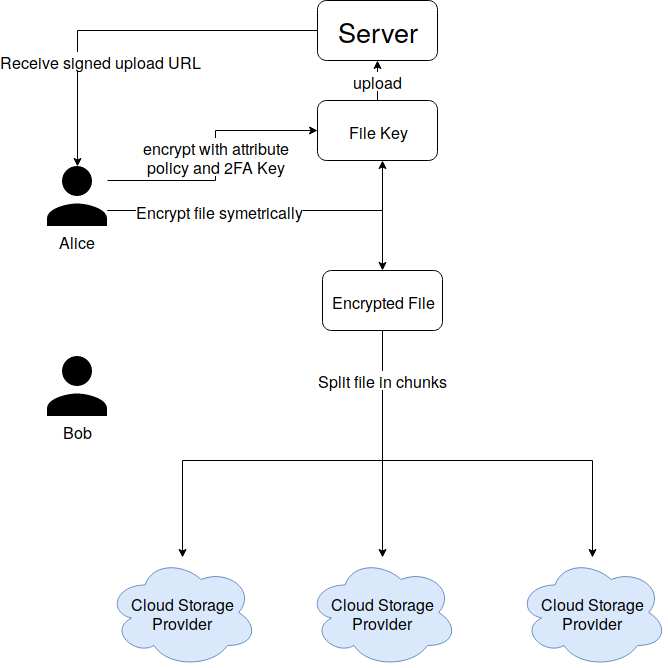
\includegraphics[width=0.7\linewidth]{img/TF-DAC-MACS-overview-encrypt.png}
    \caption{Encryption phase}
    \label{fig:tfdacmacs-encrypt}
\end{figure}

For en- and decryption we will still use the process of encrypting the file symmetrically to create a file key which will then encrypted under the attribute policy. This reduces the size of the content that will be encrypted with ABE to a minimum. Moreover, we can still benefit from the great performance of \ac{AES}. 

To upload a file encrypted under an access policy, Alice first creates the access policy (figure \ref{fig:tfdacmacs-encrypt}). In addition she is also able to encrypt the ciphertext with the authentication key she issued to Bob. \todo{Overwork graphic, might not match}. This results in a random secret $M \in G_T$. She transforms $M$ to a bit-stream and uses this as the key to encrypt the file content symmetrically. Alice uploads the ciphertext and the encrypted content to the CSP. 

\section{Decryption}
\begin{figure}[!t]
\centering
    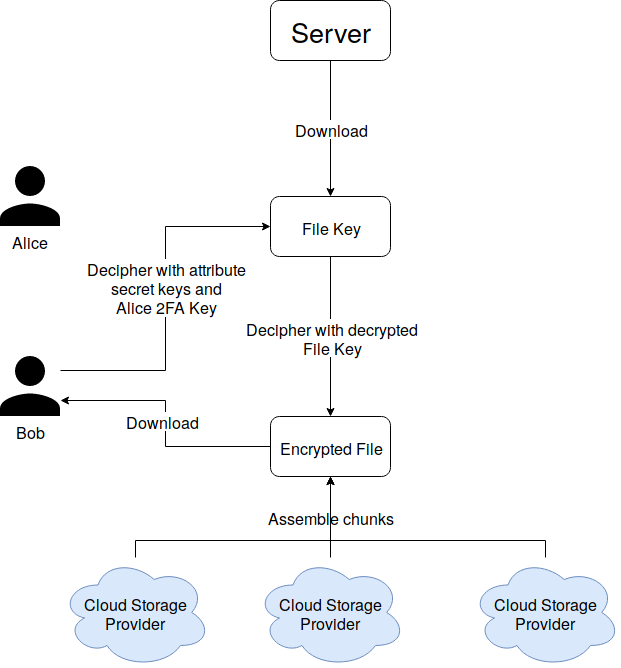
\includegraphics[width=0.7\linewidth]{img/TF-DAC-MACS-overview-decrypt.png}
    \caption{Decryption phase}
    \label{fig:tfdacmacs-decryption}
\end{figure}

On decryption first the ciphertext will be downloaded from the server. If Bob has a matching super set of attributes and the needed 2FA-Key he can recover the file key $m$ and transform it again to a bit-stream (figure \ref{fig:tfdacmacs-decryption})

Next, he downloads the encrypted file from the CSP and decrypts it with the recovered file key.

\section{Revoke attribute}
\begin{figure}[!t]
\centering
    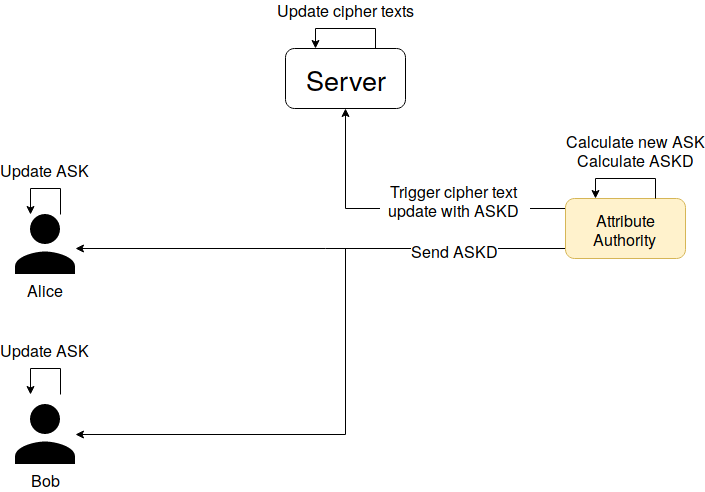
\includegraphics[width=0.7\linewidth]{img/TF-DAC-MACS-overview-revoce-attr.png}
    \caption{Attribute revocation}
    \label{fig:tfdacmacs-attr-revocation}
\end{figure}

As displayed in figure \ref{fig:tfdacmacs-attr-revocation}, a revocation of an attribute key is always triggered by the AA that administers this attribute. It first creates a new secret key for the revoked attribute and calculates for each user owning the old attribute a user-specific delta. This delta is send to each non-revoked user respectively. In addition, the AA calculates a cipher text update key. This is send to the CSP which then in turn starts updating all the cipher text for the new attribute secret key. This operation will not affect the plain text message in any kind. 

\section{Revoke two-factor key}
\begin{figure}[!t]
\centering
    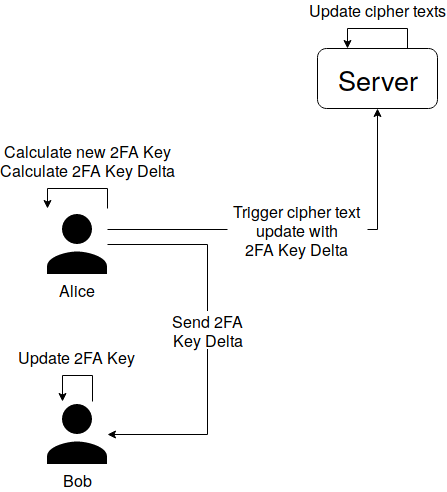
\includegraphics[width=0.6\linewidth]{img/TF-DAC-MACS-overview-revoce-user-key.png}
    \caption{Two-factor key revocation}
    \label{fig:tfdacmacs-user-auth-key-revocation}
\end{figure}

In a similar way as attributes are revoked, 2FA-Keys can be revoked. Alice, as the data owner, starts  by calculating a new two-factor key. She computes the delta to all old two-factor keys she issued and distributes them to all non-revoked users. Finally, she calculates the ciphertext update key and sends it to the CSP. The CSP updates all relevant cipher texts.

\section{Adaptions and Improvements}
While TF-DAC-MACS satisfy all the requirements it fits not perfectly. To make the scheme more usable, the fix contain that each cipher text need to be secured by a two-factor authentication was removed. In addition, the key generation of the attribute is made more dynamic. Now the attributes do not need to be known in the setup phase but can be created dynamically when an AA admin registers a user. Further, we propose a simple technique to break up TF-DAC-MACS n-of-n threshold policy in trade-off for performance. And finally we apply a technique proposed in \cite{bethencourt2007ciphertext} to implement numerical values and comparisons in boolean access formula. 

\subsection{Removing the fix two-factor contain}
To make \ac{TF-DAC-MACS} more practically applicable we removed the fixed two-factor constrain from the encryption, decryption, and cipher update phase. The two factor identifier $\alpha$ is used by the data owner to restrict the access to the content for certain users. 

This leads to the fact that the underlying \ac{ABE} schemes looses some of it expressiveness. The zero knowledge of the data owner on which individual is able to decrypt the cipher text is broken with the two factor part. Here each user, who wants to decrypt the encrypted content, needs to make an \textit{authentication request} to the data owner to receive the corresponding decryption key. To restore the possibility to let an unknown user group decrypt the cipher text, we make the two factor part optional. To do so we adapted encryption, decryption and cipher text update. The authentication key update will be ignored since it makes no sense to apply it on a non existing authentication key. 

\begin{itemize}
\item \textbf{Encryption:} 
We only need to update the $C_3$ part of the cipher text since it is the only one containing the two factor component $\alpha$.

The original $C_3$:
$$
C_3 = \Big( \prod_{v_{aid_{i}, j}\in W} g^{y_{aid_{i}, j}} \Big)^{s + \alpha} 
$$
is adapted to:
$$
\widehat{C}_3 = \Big( \prod_{v_{aid_{i}, j}\in W} g^{y_{aid_{i}, j}} \Big)^s
$$ 
In addition we will remove $oid$ from the ciphertext description since it referrers to the data owner ID which is only needed on authentication key update.

\item \textbf{Decryption:}
$SK_W = \prod_{v_{aid_i,j} \in W} SK_{v_{aid_i,j}}$ and $UPK_W = \prod_{v_{aid_i,j} \in W} UPK_{v_{aid_i,j}}$ remain defined in the same was as defined in the paper. 

On decryption the user does not need to generate $UPK_W$ and $SK_{uid, oid}$ anymore. The decryption equation is updated to:

$$
m = \frac{C_1 \cdotp e(H(uid), \widehat{C}_3)}{e(C_2, SK_W)}
$$

Note that the original decryption equation results in the above equation when the two factor part is deducted.

\begin{equation}
\begin{split}
m &= \frac{C_1 \cdotp e(H(uid), C_3)}{e(C_2, SK_W)e(SK_{uid, oid}, UPK_W)} \\
  &= \frac{C_1 \cdotp e\Big(H(uid), \Big( \prod_{v_{aid_{i}, j}\in W} g^{y_{aid_{i}, j}} \Big)^{s + \alpha} \Big)}{e(C_2, SK_W)e(H(uid)^\alpha, \prod_{v_{aid_i,j} \in W} UPK_{v_{aid_i,j}})} \\
  &= \frac{C_1 \cdotp e\Big(H(uid), \Big( \prod_{v_{aid_{i}, j}\in W} g^{y_{aid_{i}, j}} \Big)^{s + \alpha} \Big)}{e(C_2, SK_W)e(H(uid)^\alpha, \prod_{v_{aid_i,j} \in W} g^{y_{aid_i,j}})} \\
  &= \frac{C_1 \cdotp e\Big(H(uid), \Big( \prod_{v_{aid_{i}, j}\in W} g^{y_{aid_{i}, j}} \Big) \Big)^{s + \alpha}}{e(C_2, SK_W)e(H(uid), \prod_{v_{aid_i,j} \in W} g^{y_{aid_i,j}})^\alpha} \\
  &= \frac{C_1 \cdotp e\Big(H(uid), \Big( \prod_{v_{aid_{i}, j}\in W} g^{y_{aid_{i}, j}} \Big) \Big)^{s}}{e(C_2, SK_W)} \\
  &= \frac{C_1 \cdotp e\Big(H(uid), \Big( \prod_{v_{aid_{i}, j}\in W} g^{y_{aid_{i}, j}} \Big)^{s} \Big)}{e(C_2, SK_W)} \\
  &= \frac{C_1 \cdotp e(H(uid), \widehat{C}_3)}{e(C_2, SK_W)}
\end{split}
\label{eq:2faRemoval}
\end{equation}

As shown, no security is threatened since we end up at the same equation as we would if we had the two factor part included. 

\item \textbf{Attribute revocation:}
The cipher text update key is adapted from

$$
CUK^{ID_W}_{v_{aid_i,j}} = (g^s \cdotp g^\alpha)^{y'_{aid_i,j} - y_{aid_i,j}}
$$

to 

$$
\widehat{CUK}^{ID_W}_{v_{aid_i,j}} = (g^s)^{y'_{aid_i,j} - y_{aid_i,j}}
$$

$\widehat{C}'_3$ now computes as 

\begin{equation}
\begin{split}
\widehat{C}'_3 &= \widehat{C}_3 \cdotp \widehat{CUK}^{ID_W}_{v_{aid_i,j}} \\
&\cdotp \Big( \prod_{v_{aid_{t}, j}\in W, v_{aid_t, j} \neq v_{aid_i,j}} g^{y_{aid_{i}, j}} \Big)^{r} \cdotp (g^{y'_{aid_i,j}})^{r} \\
&= \Big( \prod_{v_{aid_{t}, j}\in W, v_{aid_t, j} \neq v_{aid_i,j}} g^{y_{aid_{i}, j}} \Big)^{s + r} \cdotp (g^{y'_{aid_i,j}})^{s + r}
\end{split}
\end{equation}

It can be shown that $C'_3$ computes to the message $m$ in the same way as shown in equation \ref{eq:2faRemoval}.

\item \textbf{Authentication update:}
Nothing need to change since cipher text do not contain authentication components. 
\end{itemize}

\subsection{Dynamic Secret Key Generation}
Another small adaptation in the \ac{TF-DAC-MACS} scheme was that the attributes for each \ac{AA} does not have to be known on AA initialization. They can as well be created on each users key generation. This reduces the universe of possible attribute values to thous who are actually needed.

\section{Extension To DNF-Policy}
One big advantage of TF-DAC-MACS is its constant size cipher text. It archives this by only allowing n-of-n threshold policy. This means that a data owner is only allowed to create \textit{AND} policies to encrypt his content. However, extending this scheme to n-of-m threshold policy is not trivial. To not break any security constrains we decided to just upload multiple versions of the same cipher text encrypted under different policies. Now, an user only needs to decipher one version of the cipher text to recover the encrypted content. 

Using this approach we enable access policies in disjunctive normal form (DNF) for the trade-off of linear cipher text overhead and linear overhead on cipher text updates (both scaling with the number of disjunctions).

\section{Numerical Attributes}
As described in \cite{bethencourt2007ciphertext} we could display numeric values in binary. Each number $x$ is composed of $\lceil log_2(x) \rceil$ attributes. Each of this attributes relate to either a $1$ or $0$ in one position in the binary number representation of $x$. So for example the number $5$ in binary would be displayed as $0101$ and its attribute would be: $x:0***$, $x:*1**$, $x:**0*$ and $x:***1$. 

If a user now wants to create a policy where he challenges a number $x$ to be greater or equal to $3$ he creates a policy: "$(x:1*** or (x:*1** or (x:**1* and x:***1))$". Analogous the policy for $x$ smaller than $4$: "$(x:0*** and (x:*0** or (x:*1** and x:**0* and x:***0))$".

Disadvantage of this representation is that it is limited in space. To display a 32-bit number we must issue 64 attribute values and maintain 64 attribute value keys. 


\section{Technologies}
To develop the first prototype of the system defined previously we will use the following technology stack:

\begin{itemize}
  \item \textbf{Spring boot}
  \item \textbf{Docker}
  \item \textbf{jPBC} \cite{ISCC:DecIov11}
  \item \textbf{...}
\end{itemize}
\todo{write me}

\section{Problems}

\subsection{En- and decrypting arbitrary data}
TF-DAC-MACS takes as an input for encryption a message $M \in GT$. Since there is not easy way to reconstruct a message from an element in $G_T$, we have to combine some encryption techniques to encrypt arbitrary data. 

The algorithm first chooses a random $M \in GT$ and outputs $M$ together with the constructed cipher text. $M$ is then hashed into a byte buffer using \ac{SHA}-256. In the next step we will encrypt our arbitrary data using \ac{AES} and as the key the previous computed hash. 

On decryption we first reconstruct $M$ using the ABE decryption technique and then hashing $M$ again to reconstruct our AES secret key. 